
\section{Introduction}

	\footnote{This section mostly(The information of for this section was) taken from SHiP Technical Proposal (TP) document \cite{ship_TP} just to overview the experiment and prepare reader for subsequent work under separate part of detector.}
	The completion of the particle content of the Standard Model (SM) with the discovery of the Higgs boson, and advances in cosmology highlight the necessity for a new level of understanding of physics Beyond the Standard Model (BSM). At the same time, neither experiment nor theory provide clear hints of the nature or the scale of this new physics.

	Over the next decades the Fermi-mass scale, and even beyond, will be comprehensively  explored either directly by ATLAS and CMS at the LHC, or indirectly, assuming generic couplings, at experiments like LHCb, Belle2 and NA62 \cite{NA62_TDR}. Hidden particles, which interact very weakly with the SM particles, are predicted in many theoretical models capable of explaining the shortcomings of the SM. A large part of their accessible parameter space remains unexplored. 

	In this situation SHIP is a recently proposed new general purpose fixed target facility at the SPS which is aimed at exploring the domain of hidden particles and make measurements with tau neutrinos. Hidden particles are predicted by a large number of models beyond the Standard Model. The high intensity of the SPS 400 GeV beam allows probing a wide variety of models containing light long-lived exotic particles with masses below 10 GeV/c$^2$, including very weakly interacting low-energy SUSY states.
	
		
	\subsection{Overview of the Experiment}
	At the energy accessible at the SPS, the hidden particles are predominantly produced in decays of hadrons, in particular in decays of charmed and beauty hadrons above the kaon mass, and in proton bremsstrahlung.

	\begin{figure}[!h]
	\centering
	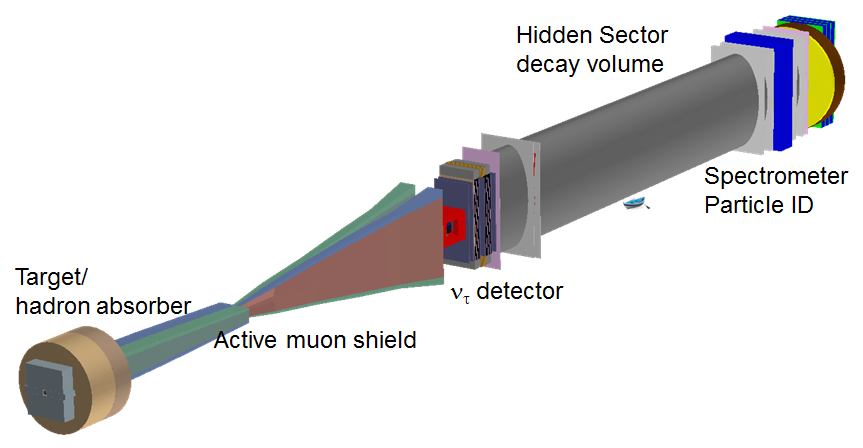
\includegraphics[width=0.9\textwidth]{SHiP-facility-overview}
	\caption{Overview of the SHiP facility \cite{ship_TP} }
	\label{fig:detector-overwiew}
	\end{figure}
	
	The detector for the direct detection of the hidden particles is designed to fully reconstruct their exclusive decays. Table \ref{table:req_decaymodes} summarizes the main decay modes of the hidden particles in the various models considered.
	
	\begin{table}[htb]
\begin{center}
\caption{Summary of the main decay modes of hidden particles in various models ($\ell = e, \mu$).}
\label{table:req_decaymodes}
\vspace{2mm}
\begin{tabular}{ll}
\hline
Models                         	& Final states              \\
\hline
Neutrino portal, SUSY neutralino                 & $\ell^{\pm}\pi^{\mp}, \ell^{\pm} K^{\mp}, \ell^{\pm}\rho^{\mp},\,\,\,\,\, \rho^{\pm}\rightarrow \pi^{\pm}\pi^0$ \\
Vector, scalar, axion portals, SUSY sgoldstino   & $\ell^+\ell^-$ \\
Vector, scalar, axion portals, SUSY sgoldstino   & $\pi^+\pi^-, K^+K^-$ \\
Neutrino portal ,SUSY neutralino, axino          & $\ell^+\ell^-\nu$ \\
Axion portal, SUSY sgoldstino                    & $\gamma\gamma$ \\
% Axino ?                                          & $\gamma$... \\ 
SUSY sgoldstino                                  & $\pi^0\pi^0$ \\
\hline
\end{tabular}
\end{center}
\end{table}

	The principal background to the hidden particle decay signal originates from the inelastic scattering of neutrinos and muons in the vicinity of the detector producing long-lived particles.
	
	The beam line is designed to minimize the background sources. The proton
interaction in the target gives rise to a copious direct production of short-lived resonances, pions and kaons. While a hadron stopper of a few metres of iron is sufficient to absorb the hadrons and the electromagnetic radiation emerging from the target, the decays of pions, kaons and short-lived resonances result in a large flux of muons and neutrinos. In order to reduce the flux of neutrinos, in particular the flux of muon neutrinos and the associated muons, the pions and kaons should be stopped as efficiently as possible before they decay. The target must therefore be made of a material with the shortest possible interaction length and be sufficiently long to contain the hadronic showers with minimum leakage. Since the production angle of the  hidden particles is relatively large, there is no requirement to minimize the beam spot.

	The short-lived resonances and the residual flux of decaying pions and kaons still give rise to a large flux of muons. This flux must be efficiently cleared from the detector fiducial volume by either a passive shield or through an active shield based on magnetic deflection. The residual flux should also be low enough so not to compromise the occupancy limit in the tau neutrino detector. As illustrated in Figure \ref{fig:detector-overwiew}, in the baseline design a 5 m horizontally wide region respecting these requirements has been achieved with a 48 m long active muon shield based on magnetic deflection of the muons in the horizontal plane.
	 
	The muon shield is followed by the 10 m long tau neutrino detector, which puts the start of the HS decay volume at about 64 m \cite{ship_TP}. The main purpose of the tau neutrino detector is to perform the first direct observation of the $\overline{\nu}_\tau$, and to study the properties and the cross section of $\nu^\tau$ and $\overline{\nu}_\tau$.
 The current optimization of muon shield and cost, results in a decay volume with an elliptical shape of 5 m width and 10 m height. The length of the decay volume is obtained by maximizing the acceptance to the hidden particle decay products given the transversal size.

	The full reconstruction of the hidden particle decays requires a magnetic spectrometer and a system for particle identification at the end of the decay volume.
	
	The particle identification system requires an electromagnetic calorimeter for $e / \gamma$ identification with sufficient granularity and energy resolution in order to reconstruct $\pi^0$'s, and a hadron calorimeter in combination with a muon detector for $ \pi / \mu$ separation.
	
	\begin{figure}[!h]
	\centering
	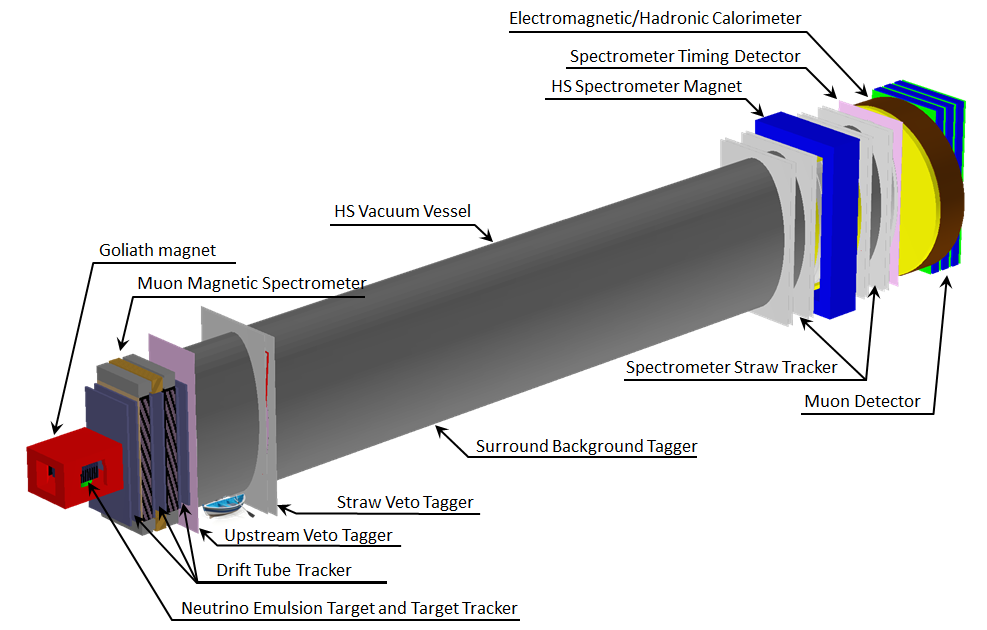
\includegraphics[width=\textwidth]{SHiP-detector-overview}
	\caption{SHiP detector layout}
	\end{figure}
	
	\subsection{Spectrometer tracker}
	
	Spectrometer tracker is a part of particle identification system.  The purpose of the HS spectrometer is to reconstruct with high efficiency the tracks of charged particles from the decay of hidden particles. The spectrometer must provide an accurate determination of the track momentum and of the flight direction within the fiducial decay volume.
	
	\begin{figure}[h!]
		\centering
		\subfloat[Position of the tracking stations and dipole magnet, overlaid with magnetic field component $B_x$ as a function of z.]{
			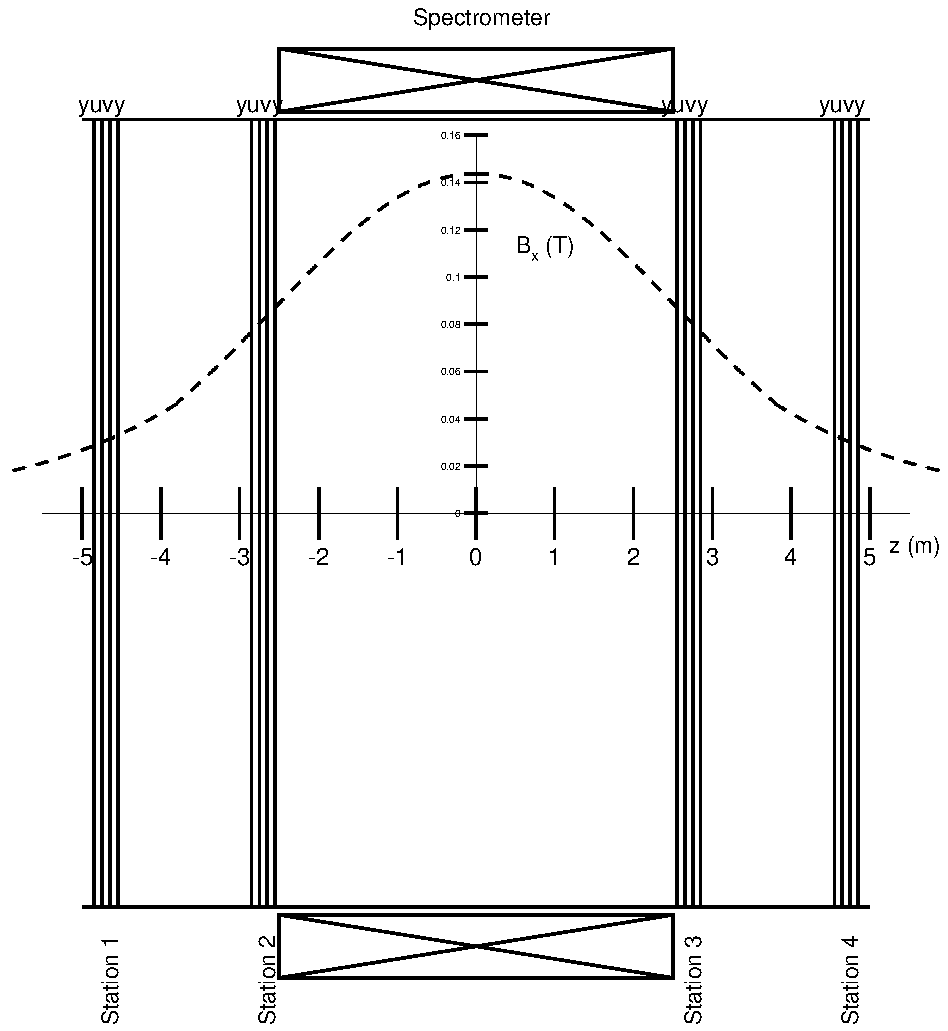
\includegraphics[width=0.50\textwidth]{spectrometer-layout} 
			\label{fig:spectrometer_layout} }%
		\qquad
		\subfloat[Four views in one station (not all straws shown, for the sake of clarity). The nominal acceptance, defined by the vacuum vessel, is shown as a red ellipse.]{
			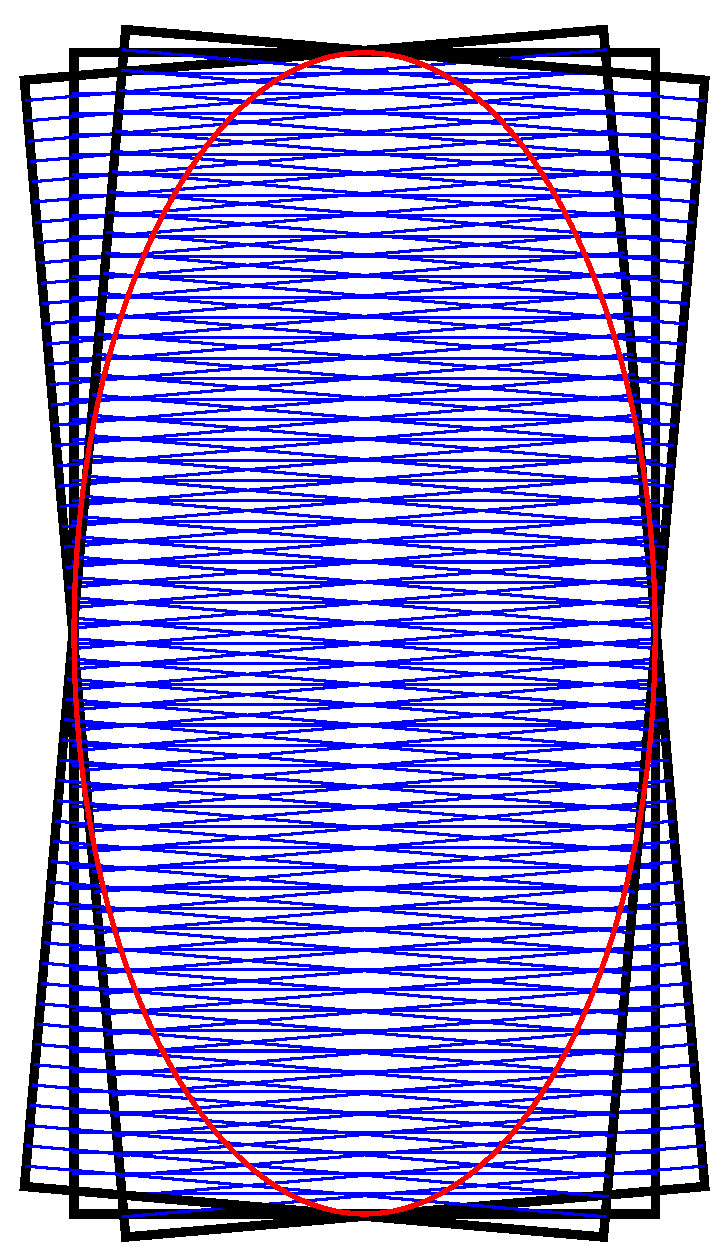
\includegraphics[width=0.4\textwidth]{straw-views.pdf} 
			\label{fig:cluster_distrib} }%
		\caption{Spectrometer layout}
	\end{figure}

	
	The spectrometer consists of a large aperture dipole magnet and two tracking telescopes on each side of the magnet. A layout with four tracking stations
symmetrically arranged around the dipole magnet, as depicted in Figure \ref{fig:spectrometer_layout}, is taken as a baseline. The size and layout of the tracker stations is connected to the size of the magnet. A dipole spectrometer magnet with a horizontal gap of 5 m, a height of 10 m and a length of 5 m provides good acceptance coverage and is considered feasible at a reasonable cost.

	Following the direction of the magnetic field, the measuring elements are oriented horizontally to measure precisely the vertical (Y) coordinate. Two stereo views (U and V) are rotated by an angle $ \pm \theta _{stereo}$ for measuring the transverse coordinate X with an accuracy degraded by $ \sim 1/ \sin \theta _{stereo}$. The precision in X (i.e. the value of the stereo angle) is driven by the need of a good enough measurement of the decay vertex, opening angle of the daughter particles (which enters the invariant mass) and impact parameter at the production target. Each station contains 4 views (Y-U-V-Y). The two stations on the same side of the magnet are separated by $\bigtriangleup = 2 m$ and a gap of $5 m$ is left between the second and third stations (i.e. each is $2.5 m$ away from the centre of the magnet).
	
	The tracking stations of the magnetic spectrometer must provide good spatial resolution and minimise the contribution from multiple scattering. In addition, the tracker must operate in vacuum. A straw tracker made of thin polyethylene terephthalate (PET) tubes is ideal to meet these goals. Gas tightness of these tubes has been demonstrated in long term tests and the mass production procedure is also well established (see NA62 experiment \cite{NA62_TDR}). The main differences between the SHiP tracker and the NA62 tracker are the need for $5 m$ long straws (vs 2.1 m in NA62). The main changes with respect to the Expression of Interest \cite{EoI} follow from the changes applied to the spectrometer magnet. The straw orientation has been turned from vertical to horizontal and one transverse dimension has been increased from 5 to 10 m.
	